\documentclass[a4paper, 12pt]{article}%тип документа

%Русский язык
\usepackage[T2A]{fontenc} %кодировка
\usepackage[utf8]{inputenc} %кодировка исходного кода
\usepackage[english,russian]{babel} %локализация и переносы

%отступы 
\usepackage[left=2cm,right=2cm,top=2cm,bottom=3cm,bindingoffset=0cm]{geometry}

%Вставка картинок
\usepackage{graphicx}
\graphicspath{}
\DeclareGraphicsExtensions{.pdf,.png,.jpg, .jpeg}

%Таблицы
\usepackage[table,xcdraw]{xcolor}
\usepackage{booktabs}

%Графики
\usepackage{pgfplots}
\pgfplotsset{compat=1.9}

%Математика
\usepackage{amsmath, amsfonts, amssymb, amsthm, mathtools}

%Заголовок
\author{Нугманов Булат \\ группа 827}
\title{Работа 1.4.8 \\ Измерение модуля Юнга методом 
акустического резонанса}

\begin{document}
\maketitle
\tableofcontents
\newpage
\section{Цель работы}
Исследование явления акустического резонанса. Измерение скорости
распространения продольных колебаний в тонких стрежнях. Измерение модуля Юнга различных материалов. 
\section{Оборудование}
Генератор звуковых частот, частотомер, осциллограф,
электромагнитные излучатель и приемник колебаний, набор стержней из различных материалов (стали, алюминия, меди).
\section{Отчёт о работе}
\subsection{Общая теория}
\subsubsection{Распространение продольных волн в тонких стержнях}
Распространение продольных волн в тонких стержнях 
Акустические волны, распространяющиеся в металлических стержнях,
существенно отличаются от волн в неограниченной среде. Строгий анализ
распространения таких волн связан с довольно громоздкими математическими
расчетами. Будем рассматривать волны, длина $\lambda$ которых велика по
сравнению с радиусом $R$ стержня. Опишем распространение продольной
волны вдоль оси тонкого стержня постоянного сечения площадью $S$ .
Стержень считается тонким в том случае, когда радиус стержня $R$ мал по
сравнению с длиной волны $\lambda$, т.е. $R/\lambda\ll 1$.

Направим ось x вдоль геометрической оси стержня (рис. 1).
\begin{figure}[h!]
\center{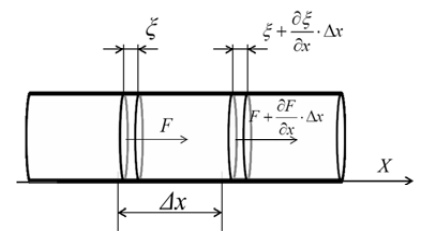
\includegraphics[scale=1.5]{2.jpg}}
\caption{Силы, действующие на элемент стержня при продольных колебаниях}
\end{figure}
Под действием
продольной силы $F$ элементарный отрезок стержня $\Delta x$ , ограниченный
плоскостями $\Delta x$ и $(x+\Delta x)$, растянется или сожмется на величину $\Delta\xi=\dfrac{\partial \xi}{\partial x}\Delta x$, где $\dfrac{\partial\xi}{\partial x}$ — относительное удлинение, т. е. деформация элемента стержня. Напряжение $\sigma$ (т. е. сила, действующая на единицу поперечного
сечения стержня) согласно закону Гука равно
\begin{equation}
\sigma=\frac{F}{S}=E\dfrac{\partial \xi}{\partial x}.
\end{equation}
Коэффициент пропорциональности $E$ носит название модуля Юнга и имеет размерность Н/м2. В результате переменной деформации вдоль оси стержня будет распространяться
продольная волна. Действительно, в сечениях $x$ и $x+\Delta x$
напряжения будут различными, а их разность можно записать следующим
образом: 
\begin{equation}
\sigma(x+\Delta x)-\sigma(x)=\frac{1}{S}\dfrac{\partial\xi}{\partial x}\Delta x=\frac{\partial}{\partial x}\left(\frac{F}{S}\right)\Delta x.
\end{equation}
Эта разность напряжений вызовет движение элемента стержня массой
$m=S\rho\Delta x$ вдоль оси $x$ ($\rho$ — плотность материала стержня). Используя
соотношения (1) и (2), на основании второго закона Ньютона уравнение
движения этого элемента можно записать в виде: 
\begin{equation}
S\rho\Delta x\dfrac{\partial^2\xi}{\partial t^2}=SE\dfrac{\partial^2\xi}{\partial x^2}\Delta x.
\end{equation}
Обозначив $E/\rho$ через $c^2_{\text{ст}}$, выражение (3) запишем в следующем виде: 
\begin{equation}
\dfrac{\partial^2\xi}{\partial t^2}=c^2_{\text{ст}}\dfrac{\partial^2\xi}{\partial x^2}.
\end{equation}
Это уравнение носит название волнового  уравнения. Оно, в частности,
описывает распространение продольных волн в стержне. Общее решение
волнового уравнения можно представить в форме двух бегущих волн, распространяющихся в обе стороны вдоль оси $x$ со скоростью
$c^2_{\text{ст}}$ :
\begin{equation}
\xi(x,t)=f(c_{\text{ст}}t-x)+g(c_{\text{ст}}t+x),
\end{equation}
где $f$ и $g$ — произвольные функции (определяемые начальными и граничными
условиями).
Параметр $c_{\text{ст}}$ в выражениях (4) и (5) имеет смысл скорости распространения волны. В рассматриваемом нами случае $R/\lambda\rightarrow 0$ скорость распространения
упругой продольной волны стремится к величине
\begin{equation}
c_{\text{ст}}\approx\sqrt{\dfrac{E}{\rho}}.
\end{equation}
В данной работе исследуются именно такие волны. \\
Отметим, что в высокочастотном (т. е. коротковолновом) пределе
при $\lambda\ll R$ скорость акустических волн в стержне стремится к скорости продольных волн в неограниченной среде ($\mu$ — коэффициент Пуассона): 
\begin{equation}
c_{\text{i}}=\sqrt{\dfrac{E(1+\mu)}{\rho(1+\mu)(1-2\mu)}}.
\end{equation}
\subsubsection{Собственные колебания стержня}
В случае гармонического возбуждения колебаний с частотой $f$ продольная волна в тонком стержне может быть представлена в виде суперпозиции двух бегущих навстречу друг другу синусоидальных волн:
\begin{equation}
\xi(x,t)=A_1\sin(\omega t-kx+\varphi_1)+A_2\sin(\omega t+kx+\varphi_1),
\end{equation}
где $\omega=2\pi f$ — циклическая частота, коэффициент $k=2\pi/\lambda$ называют волновым числом или пространственной частотой. Здесь первое слагаемое описывает волну, бегущую в положительном направлении по оси $x$ , второе
— в отрицательном. Скорость их распространения равна
\[c_{\text{ст}}=\omega/k.\]
Несложно показать, что при отражении синусоидальной волны от свободного конца стержня, её фаза не изменяется. Тогда
\begin{equation}
L=n\frac{\lambda_{\text{n}}}{2}.
\end{equation}
Таким образом, на длине стержня должно укладываться целое число полуволн.
\subsubsection{Измерение скорости распространения  
продольных волн в стержне}
Зная плотность материала и величину скорости $c_{\text{ст}}$ можно по формуле (6) вычислить модуль Юнга материала $E$ . Для определения скорости $c_{\text{ст}}$ в данной работе используется метод акустического резонанса. Это явление состоит в том, что при частотах гармонического возбуждения, совпадающих с собственными частотами колебаний стержня $f\approx f_{\text{n}}$ , резко
увеличивается амплитуда колебаний, при этом в стержне образуется стоячая волна.
В данной работе возбуждение колебаний происходит посредством воздействия
на торец стержня периодической силой, направленной вдоль его
оси. Зная номер гармоники $n$ и частоту $f_{\text{n}}$, на которой наблюдается резонансное
усиление амплитуды колебаний, вызванных периодическим воздействием
на торец стержня, можно рассчитать скорость распространения
продольных волн в стержне:
\begin{equation}
c_{\text{ст}}=f_{\text{n}}\lambda_{\text{n}}=\dfrac{2Lf_{\text{n}}}{n}.
\end{equation}
Таким образом, для того, чтобы измерить скорость $c_{\text{ст}}$, нужно измерить частоты резонансных гармоник для различных $n$, и зная геометрические размеры стержня, рассчитать скорость по формуле (15). Далее, по формуле (6) можно рассчитать и модуль Юнга материала, из которого изготовлен стержень. Этот метод определения модуля Юнга материала является одним из самых точных. 
\subsubsection{Описание экспериментальной установки}
\begin{figure}[h!]
\center{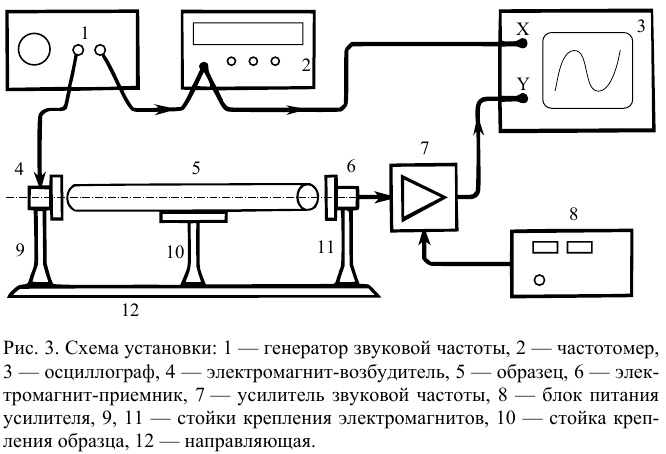
\includegraphics[scale=1]{1.jpg}}
\caption{Установка с описанием}
\end{figure}
\subsection{Снятие эскпериментальных данных}
Для начала мы собрали экспериментальную установку так как, показано в предыдущем разделе. После подготовления всех элементов и настройки осциллографа мы приступили к снятию экспериментальных данных. Для каждого стержня данные представлены в отдельном пункте.
\subsubsection{Медь}
\paragraph*{Размер 1}
Линейные размеры представлены с помощью этой таблицы:
\begin{table}[h]
\center{\begin{tabular}{|l|l|l|l|l|}
\hline
Медь1 & $L$, mm & $d$, mm & $M$, gr & $V$, $cm^3$ \\ \hline
Значение         & 605     & 12,0    & 636,34  & 68,424                     \\ \hline
Погрешность      & 1       & 0,2     & 0,3     & 0,024                      \\ \hline
\end{tabular}}
\end{table}
\\Исходя из этого, плотность стержня:
\begin{equation}
\rho=(9,30\pm0,01)gr/cm^3.
\end{equation}
На данной талице представлена зависимость частоты резонанса для соответсвтвенных гармоник:
\begin{table}[h]
\center{\begin{tabular}{|l|l|l|l|l|l|}
\hline
$n$     & 1      & 2      & 3      & 4     & 5       \\ \hline
$f$, Hz & 3214,7 & 6444,8 & 9646,4 & 12884 & 16048,4 \\ \hline
\end{tabular}}
\end{table}
\paragraph*{Размер 2}
Линейные размеры представлены с помощью этой таблицы:
\begin{table}[h]
\center{\begin{tabular}{|l|l|l|l|l|}
\hline
Медь2 & $L$, mm & $d$, mm & $M$, gr & $V$, $cm^3$ \\ \hline
Значение         & 532     & 10,0    & 375,1  & 41,78                     \\ \hline
Погрешность      & 1       & 0,2     & 0,3     & 0,03                      \\ \hline
\end{tabular}}
\end{table}
\\Исходя из этого, плотность стержня:
\begin{equation}
\rho=(8,98\pm0,02)gr/cm^3.
\end{equation}
На данной талице представлена зависимость частоты резонанса для соответсвтвенных гармоник:
\begin{table}[h]
\center{\begin{tabular}{|l|l|l|l|l|l|}
\hline
$n$     & 1      & 2      & 3      & 4     & 5       \\ \hline
$f$, Hz & 3804,4 & 7606 & 11391,3 & 15234,2 & 19005 \\ \hline
\end{tabular}}
\end{table}
\subsubsection{Сталь}
\paragraph*{Размер 1}
Линейные размеры представлены с помощью этой таблицы:
\begin{table}[h]
\center{\begin{tabular}{|l|l|l|l|l|}
\hline
Сталь1 & $L$, mm & $d$, mm & $M$, gr & $V$, $cm^3$ \\ \hline
Значение         & 605     & 12,2    & 545,43  & 70,724                     \\ \hline
Погрешность      & 1       & 0,2     & 0,3     & 0,026                      \\ \hline
\end{tabular}}
\end{table}
\\Исходя из этого, плотность стержня:
\begin{equation}
\rho=(7,712\pm0,008)gr/cm^3.
\end{equation}
На данной талице представлена зависимость частоты резонанса для соответсвтвенных гармоник:
\begin{table}[h!]
\center{\begin{tabular}{|l|l|l|l|l|l|}
\hline
$n$     & 1      & 2      & 3      & 4     & 5       \\ \hline
$f$, Hz & 4127,4 & - & 12380,6 &16556,4 & 20602,2 \\ \hline
\end{tabular}}
\end{table}
\paragraph*{Размер 2}
Линейные размеры представлены с помощью этой таблицы:
\begin{table}[h!]
\center{\begin{tabular}{|l|l|l|l|l|}
\hline
Сталь2 & $L$, mm & $d$, mm & $M$, gr & $V$, $cm^3$ \\ \hline
Значение         & 401     & 8,0    & 157,53  & 20,16                     \\ \hline
Погрешность      & 1       & 0,2     & 0,3     & 0,03                      \\ \hline
\end{tabular}}
\end{table}
\\Исходя из этого, плотность стержня:
\begin{equation}
\rho=(7,81\pm0,03)gr/cm^3.
\end{equation}
На данной талице представлена зависимость частоты резонанса для соответсвтвенных гармоник:
\begin{table}[h!]
\center{\begin{tabular}{|l|l|l|l|l|l|}
\hline
$n$     & 1      & 2      & 3      & 4     & 5       \\ \hline
$f$, Hz & 6438,6 & 12885 & 19317 & 25749 & 32142 \\ \hline
\end{tabular}}
\end{table}
\subsubsection{Дюраль}
\paragraph*{Размер 1}
Линейные размеры представлены с помощью этой таблицы:
\begin{table}[h!]
\center{\begin{tabular}{|l|l|l|l|l|}
\hline
Дюраль1 & $L$, mm & $d$, mm & $M$, gr & $V$, $cm^3$ \\ \hline
Значение         & 604     & 11,8    & 192,04  & 66,053                     \\ \hline
Погрешность      & 1       & 0,2     & 0,3     & 0,025                      \\ \hline
\end{tabular}}
\end{table}
\\Исходя из этого, плотность стержня:
\begin{equation}
\rho=(2,907\pm0,006)gr/cm^3.
\end{equation}
На данной талице представлена зависимость частоты резонанса для соответсвтвенных гармоник:
\begin{table}[h!]
\center{\begin{tabular}{|l|l|l|l|l|l|}
\hline
$n$     & 1      & 2      & 3      & 4     & 5       \\ \hline
$f$, Hz & 4244,5 & 8495 & 12730 & 16976 & 21204 \\ \hline
\end{tabular}}
\end{table}
\paragraph*{Размер 2}
Линейные размеры представлены с помощью этой таблицы:
\begin{table}[h!]
\center{\begin{tabular}{|l|l|l|l|l|}
\hline
Дюраль2 & $L$, mm & $d$, mm & $M$, gr & $V$, $cm^3$ \\ \hline
Значение         & 436     & 9,9    & 93,451  & 33,562                     \\ \hline
Погрешность      & 1       & 0,2     & 0,3     & 0,036                      \\ \hline
\end{tabular}}
\end{table}
\\Исходя из этого, плотность стержня:
\begin{equation}
\rho=(2,782\pm0,012)gr/cm^3.
\end{equation}
На данной талице представлена зависимость частоты резонанса для соответсвтвенных гармоник:
\begin{table}[h!]
\center{\begin{tabular}{|l|l|l|l|l|l|}
\hline
$n$     & 1      & 2      & 3      & 4     & 5       \\ \hline
$f$, Hz & 5834,9 & - & - & - & - \\ \hline
\end{tabular}}
\end{table}
\paragraph*{Половинный резонанс}
Для дюрали 1 размера мы так же померили частоту резонанса для "половинной гармоники". Это значение равно 2122,1 герца. Это -- фотография рисунка, получившаяся на осциллографе в момент резонанса:
\begin{figure}[h!]
\center{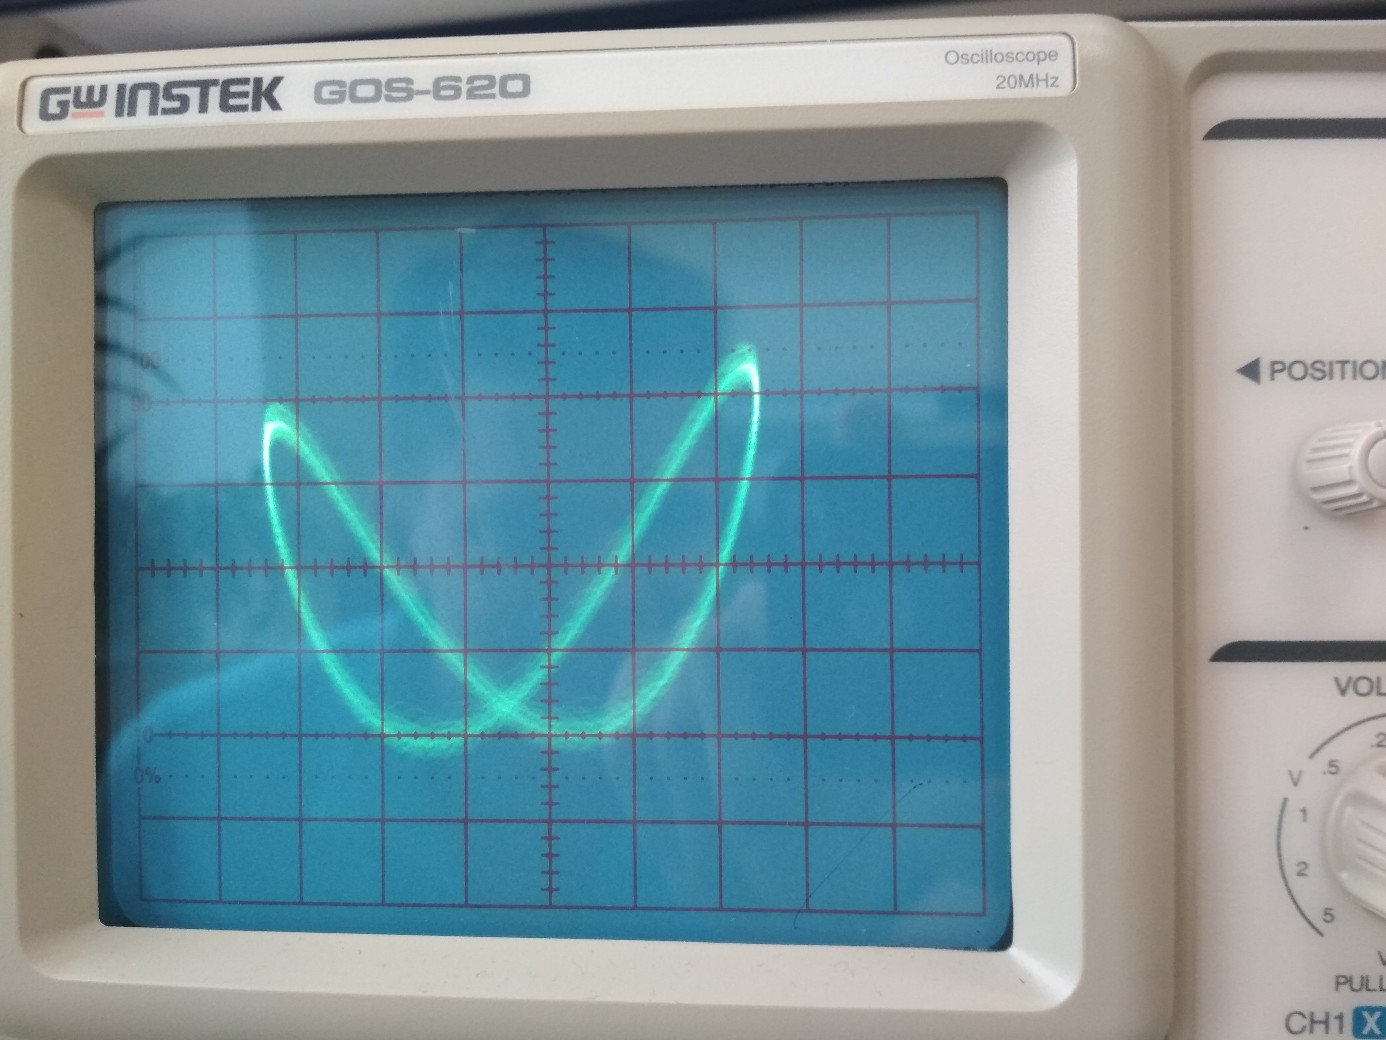
\includegraphics[scale=0.25]{fotka.jpg}}
\caption{Узор на осциллографе}
\end{figure}
Этот результат можно объяснить следующим образом: как уже было сказано ранее,  общее решение волнового уравнения можно представить в форме двух бегущих волн, распространяющихся в обе стороны вдоль оси $x$ со скоростью
$c^2_{\text{ст}}$ : 
\[\xi(x,t)=f(c_{\text{ст}}t-x)+g(c_{\text{ст}}t+x),\]
где $f$ и $g$ — произвольные функции (определяемые начальными и граничными
условиями). Далее было получено упрощенное решение этого уравнения, однако полное решение этого уравнения -- это произведение двух рядов Фурье волновой функции, и из этого уравнения получается, что при половине собственной частоты стержня для его первой гармоники все равно возникает резонанс, а фигура, показанная на фото -- это фигура Лиссажу, которая показывает, что частота волны, поступающей со стержня в 2 раза больше частоты волны, поступающей с генератора частот. Это объясняется тем же решением уравнений Фурье, из которых получается интерференция половинных волн первой гармоники, которые вместе дают резонансную частоту.
\subsubsection{Добротность}
Для измерения добротности системы, для каждого из стержней мы снимали в амплитудно-частотную характеристику $A(f-f_1)$ колебаний вблизи первого резонанса. Ширина максимума $A(f-f_n)$, как известно из теории колебаний,
связана с добротностью $Q$ стержня как колебательной системы: если $\Delta f$
— ширина амплитудно-частотной характеристики на уровне $A=\frac{A_{max}}{\sqrt{2}}$, то
\begin{equation}
Q=\frac{f}{\Delta f} 
\end{equation} 
Для каждого из стержней мы смотрели ширину пика первой гармоники. Полученные значения указаны в таблице:
\begin{table}[h]
\begin{tabular}{|ll|ll|ll|}
\hline
Медь                            &        & Сталь                          &        & Дюраль                         &         \\ \hline
\multicolumn{1}{|l|}{$f_r$, Hz} & 3214,6 & \multicolumn{1}{l|}{$f_r$, Hz} & 4127,2 & \multicolumn{1}{l|}{$f_r$, Hz} & 4242,12 \\ \hline
\multicolumn{1}{|l|}{$f_1$, Hz} & 3214,2 & \multicolumn{1}{l|}{$f_1$, Hz} & 4125,4 & \multicolumn{1}{l|}{$f_1$, Hz} & 4241,7  \\ \hline
\multicolumn{1}{|l|}{$f_2$, Hz} & 3214,8 & \multicolumn{1}{l|}{$f_2$, Hz} & 4128   & \multicolumn{1}{l|}{$f_2$, Hz} & 4242,6  \\ \hline
\multicolumn{1}{|l|}{$Q_1$}     & 8037   & \multicolumn{1}{l|}{$Q_1$}     & 2293   & \multicolumn{1}{l|}{$Q_1$}     & 10100   \\ \hline
\multicolumn{1}{|l|}{$Q_2$}     & 16073  & \multicolumn{1}{l|}{$Q_2$}     & 5157   & \multicolumn{1}{l|}{$Q_2$}     & 8838    \\ \hline
\end{tabular}
\end{table}
\\
Мы измеряли ширину пика "с двух сторон', при меньшем значении $f_1$, и большем -- $f_2$. Как видно из таблицы, погрешности такого измерения добротности уже не меньше 50\%, поэтому данные служат лишь для оценки порядка добротности нашей системы. Такая неточность в измерении савязана в первую очередь с тем, что система для выставления частоты на генераторе очень неустойчивая, а пик резонанса по ширине имеет порядок единиц Гц.
\subsection{Обработка экспериментальных данных}
Построим графики для каждого стержня размера 1.
\paragraph*{Медь}
\begin{figure}[h!]
\center{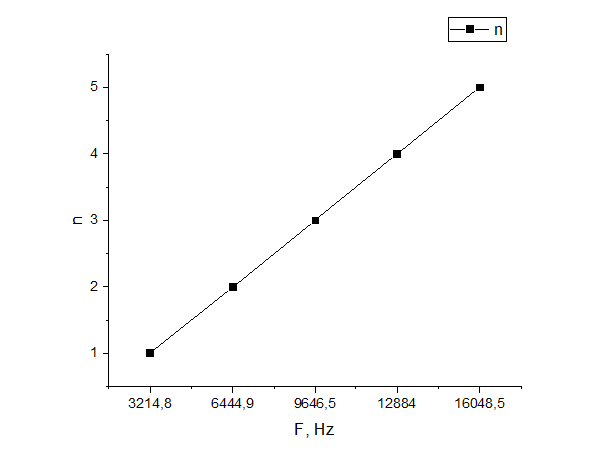
\includegraphics[scale=0.8]{grmed.png}}
\caption{Гармоники Меди}
\end{figure}
Отсюда находим $c_{\text{ст}}$:
\begin{table}[h]
\begin{tabular}{|l|l|l|l|}
\hline
$c_{\text{ст1}}$, м/с & $\sigma_{c1}$, м/с & $c_{\text{ст2}}$, м/с & $\sigma_{c2}$, м/с \\ \hline
3892                  & 15                  & 4046                  & 24 \\ \hline
\end{tabular}
\end{table}
\\
Здесь результаты для двух размеров меди.
\paragraph*{Сталь}
\begin{figure}[h!]
\center{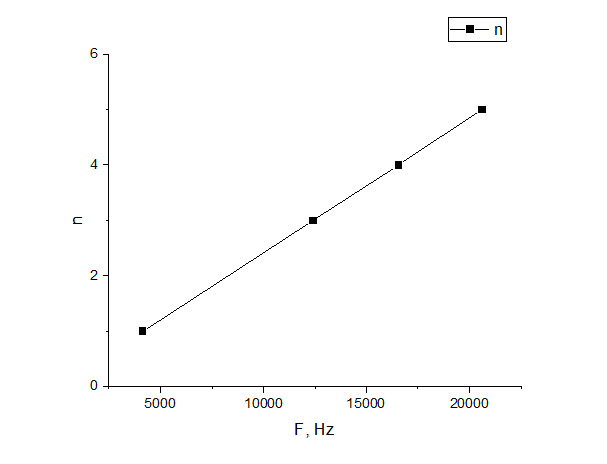
\includegraphics[scale=0.7]{grsteel.png}}
\caption{Гармоники Стали}
\end{figure}
Отсюда находим $c_{\text{ст}}$:
\begin{table}[h]
\begin{tabular}{|l|l|l|l|}
\hline
$c_{\text{ст1}}$, м/с & $\sigma_{c1}$, м/с & $c_{\text{ст2}}$, м/с & $\sigma_{c2}$, м/с \\ \hline
4995                  & 20                  & 5163                  & 26 \\ \hline
\end{tabular}
\end{table}
\\
\paragraph*{Дюраль}
\begin{figure}[h!]
\center{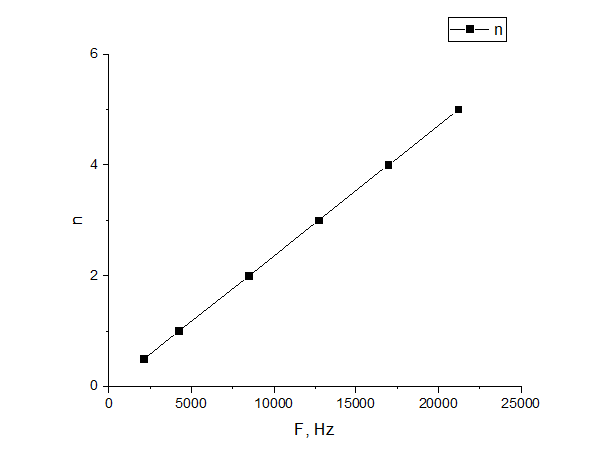
\includegraphics[scale=0.7]{grdur.png}}
\caption{Гармоники Дюрали}
\end{figure}
Отсюда находим $c_{\text{ст}}$:
\begin{table}[h!]
\begin{tabular}{|l|l|l|l|}
\hline
$c_{\text{ст1}}$, м/с & $\sigma_{c1}$, м/с & $c_{\text{ст2}}$, м/с & $\sigma_{c2}$, м/с \\ \hline
5127                  & 21                  & 5088                  & 48 \\ \hline
\end{tabular}
\end{table}
\\
Таким образом, мы можем найти модуль Юнга для каждого из стержней, воспользовавшись формулой:
\begin{equation}
E=\rho c_{\text{ст}}^2.
\end{equation}
Таким образом запишем результаты в таблицу и сравним с табличными значениями.
\begin{table}[h]
\begin{tabular}{|l|l|l|}
\hline
№         & Медь                         & Табличные данные для меди   \\ \hline
$E_1$, Па & $(1.409\pm0.012)\times10^{11}$ & $(1.30\pm0.15\times10^{11}$   \\ \cline{1-2}
$E_2$, Па & $(1.470\pm0.014)\times10^{11}$ &                             \\ \hline
№         & Сталь                        & Табличные данные для стали  \\ \hline
$E_1$, Па & $(1.924\pm0.015)\times10^{11}$ & $(2.1\pm0.1)\times10^{11}$    \\ \cline{1-2}
$E_2$, Па & $(2.082\pm0.018)\times10^{11}$ &                             \\ \hline
№         & Дюраль                       & Табличные данные для Дюраля \\ \hline
$E_1$, Па & $(0.763\pm0.009)\times10^{11}$ & $(0.73\pm0.05)\times10^{11}$  \\ \cline{1-2}
$E_2$, Па & $(0.720\pm0.010)\times10^{11}$ &                             \\ \hline
\end{tabular}
\end{table}
\\
\section{Вывод}
Таким образом мы исследовали свойства акустического резонанса и измерили модуль Юнга для трех металлов с достаточно хорошей точностью. Как видно, данные соотносятся с табличными с учетом погрешности. Многие характеристики для стержней разных размеров не совпадают, даже с учетом погрешности, из чего можно сделать вывод, что они были сделаны из разных партий сплавов, или с разной термической обработкой. Так же мы показали, что оборудование недостаточно чувствительное для того, чтобы измерить добротность системы, однако позволяет оценить ее порядок.
















\end{document}